\documentclass[11pt,a4paper]{article}
\usepackage[margin=1in]{geometry}
\usepackage{amsmath,amssymb}
\usepackage{graphicx}
\usepackage{booktabs}
\usepackage{siunitx}
\usepackage[table]{xcolor}
\usepackage{caption}
\usepackage{subcaption}
\usepackage[colorlinks=true,linkcolor=blue!55!black,urlcolor=blue!55!black,
            citecolor=blue!55!black,
            pdftitle={Tracking and Removing a Migrating Window Blemish},
            pdfauthor={CMU Skyline Monitor (Simon DeDeo, with Claude)},
            pdfsubject={Bayesian estimation and autonomous correction of a near-field optical defect},
            pdfkeywords={Bayesian inference, image correction, defocus optics, autonomous systems}]{hyperref}
\usepackage{microtype}
\usepackage{tikz}
\usetikzlibrary{positioning,arrows.meta,fit,backgrounds}

\newcommand{\Lbg}{L_{\mathrm{bg}}}
\newcommand{\Lsp}{L_{\mathrm{sp}}}
\newcommand{\code}[1]{\texttt{\small #1}}

\title{\bfseries Tracking and Removing a Migrating Window Blemish}
\author{CMU Skyline Monitor --- \code{pandr} / \code{akdeniz}}
\date{2026-07-28 (v6.3)}

\begin{document}
\maketitle

\begin{abstract}
\noindent
A $\sim\SI{0.25}{mm}$ speck on the window of a sky monitor is imaged by the camera's
$f/4$ pupil from $\sim\SI{3}{cm}$ as a \SI{76}{px}, \SIrange{2}{7}{\percent} shadow,
which contrast enhancement amplifies $\sim\!2.9\times$ in the served image. The shadow
geometry acts as a $\sim\SI{92}{px/mm}$ strain gauge: sub-millimetre thermal flexure of
sash and mount walked the feature's image \SI{120}{px} in a week, including
\SIrange{7}{18}{px} within single days. We remove it with a layered Bayesian scheme: a
hierarchical pixel model (Student-$t$ likelihood, position pinned across exposure
brackets, days tied by a drift-informed random walk) locates the feature; a nightly
recursive filter carries position and velocity forward, each estimate stamped with its
data's epoch; and at every capture a template-lock measurement update corrects the
prediction, with depth taken from a registered empirical transmittance map rather than
any parametric shape. On clean daylight frames with a detectable dip, the median
displayed artifact falls from \SI{4.5}{\percent} to \SI{0.5}{\percent} (day-blocked
95\% CI on removal: \SIrange{86}{91}{\percent}).
\end{abstract}

\begin{center}
  
\includegraphics[width=0.492\textwidth]{figs/full_before.jpg}\hfill
  
\includegraphics[width=0.492\textwidth]{figs/full_after.jpg}
  \captionof{figure}{The same three raw brackets fused without (left) and with (right)
  the correction --- 2026-07-25 19:17 EDT. The blemish is the dark smudge at the top of
  the sky, left of centre; displayed dip \SI{5.46}{\percent} $\rightarrow$
  \SI{0.77}{\percent}. The corrected fusion is the frame now served in the public
  archive.}
  \label{fig:full}
\end{center}

{\small\setcounter{tocdepth}{1}\tableofcontents}

\section{The instrument and the defect}

A \SI{4}{K} camera (\num{3840}$\times$\num{2160}) images the CMU skyline through a fixed
window. Every five minutes it captures a three-exposure bracket, fused by Mertens
exposure fusion and finished with a local-contrast pass (CLAHE) plus global saturation
and contrast curves. Brackets are archived losslessly, so all photometry runs on raw
frames; the correction is applied to the raw brackets \emph{before} fusion, because the
enhancement stage amplifies any residual dip roughly $2.9\times$, scene-dependently. The camera (Elgato Facecam 4K) is an
$f/4.0$ fixed-focus design --- Elgato Prime Lens, \SI{21}{mm} equivalent on a 1/1.8''
sensor (actual focal length $\approx\SI{4.3}{mm}$, entrance pupil
$\approx\SI{1.1}{mm}$), focus range \SIrange{30}{120}{cm} --- mounted with its lens
under \SI{1}{cm} from the pane. These numbers matter: the blemish is imaged as an
out-of-focus pupil shadow, and every inference about its physical nature runs through
them (\S\ref{sec:what}). The blemish currently projects to $\sim(1300,132)$ --- only
\SI{130}{px} below the top edge of the sensor, which constrains the correction geometry
(\S\ref{sec:physics}).

\paragraph{What is deployed and what is offline.} This note describes code in three
states, and labels each claim accordingly: \emph{deployed} (running on the capture host
\code{pandr} or the compute host \code{akdeniz} as of 2026-07-28), \emph{offline}
(analyses run to produce the results here, with code retained under
\code{spot\_paper/code/}), and \emph{proposed}. The authoritative component-by-component
table, with byte-copies of the deployed files, is \code{PRODUCTION\_STATUS.md} and
\code{production/} in the project directory. An earlier draft did not make these
distinctions and correctly drew a reviewer's objection.

\section{Statistical model and inference}
\label{sec:inference}

\subsection{Photometric model}

Per colour channel, in linear light, the blemish maps the background radiance it occludes
as an affine transformation,
\begin{equation}
  \Lsp = t\,\Lbg + s,
  \qquad\text{so the fractional dip}\qquad
  d = 1 - \Lsp/\Lbg = (1-t) - s\,\Lbg^{-1}.
  \label{eq:m1}
\end{equation}
The intercept of $d$ against $\Lbg^{-1}$ identifies the transmittance $t$; the slope is
exactly $-s$, so a nonzero slope is a direct test for an additive component (reported in
\S\ref{sec:physics}). One structural fact shapes everything: \emph{an exposure bracket
cannot separate $t$ from $s$}. Changing exposure scales $\Lsp$ and $\Lbg$ together, so
within a bracket the three points are collinear with slope $t + s/\Lbg$. Brackets
calibrate the tone curve, nothing more; separating $t$ from $s$ requires natural
variation of $\Lbg$ at fixed window irradiance (cloud behind the blemish, the twilight
ramp).

\subsection{Locating the blemish: spatial models (offline analysis)}

Equation~\eqref{eq:m1} uses scalar aperture summaries and carries no spatial
information. Two spatial estimators exist, and it matters which is which. The
\emph{production} nightly estimator (deployed, \code{spotnight.py}) is deliberately
simple: median-stacked ratio maps, position pinned across brackets, a half-depth
centroid, and a recursive prior with step and spread gates. The \emph{Bayesian pixel
model below is the offline analysis} that validates it: fitted independently, the two
agree along the whole eight-day track to $\sim\SI{3}{px}$, which is the justification
for running the cheap estimator nightly. In the offline model, a level-normalised image
window is a smooth background minus a blob,
\begin{equation}
  y_i \sim \operatorname{Student-}t\!\left(\nu,\;
    b_{0,m} + \mathbf{x}_i^{\!\top}\boldsymbol{\beta}_m
    - A_{k(m)}\, e^{-Q_i/2},\; \sigma_m\right),
  \label{eq:spatial}
\end{equation}
with $m$ indexing image stacks, $k(m)$ the exposure bracket of stack $m$ (one
amplitude per bracket class), $\mathbf{x}_i$ the quadratic basis
$(u,v,u^2,uv,v^2)$ standardised per stack, and
\begin{equation*}
  Q_i = \frac{1}{1-\rho^2}\Big[\tfrac{(u_i-c_x)^2}{\sigma_x^2}
   - \tfrac{2\rho(u_i-c_x)(v_i-c_y)}{\sigma_x\sigma_y}
   + \tfrac{(v_i-c_y)^2}{\sigma_y^2}\Big],
\end{equation*}
with priors $c_x, c_y \sim \mathcal N(0, 30)$ px about the drift-predicted centre and a
non-centred random walk of scale $\tau$ px/night tying days;
$\sigma_{x,y} \sim \mathcal N(33, 7)$ bounded to $[15,60]$ px;
$\rho \sim \mathcal N(0, 0.35)$ on $[-0.85, 0.85]$;
$A_k \sim \mathcal N(0.02, 0.012)$ bounded to $[0.002, 0.10]$ (a positive floor, see
below); Student-$t$ errors ($\nu \sim$ Gamma, $\nu \ge 2$) keep cloud edges from
dragging the centre. Exact code, bounds, seeds and the multi-start command lines are in
\code{spot\_paper/code/}. Three structural choices carry the statistical weight:

\begin{itemize}
\item \textbf{One position, shared across brackets.} The three brackets of a tick see the
  same glass at the same instant. Pinning the centre across brackets (after normalising
  each bracket's dip by its own peak, so shape is compared rather than depth) reduced
  per-bracket disagreement from $\sim\!\SI{60}{px}$ to a few px.
\item \textbf{Positions tied across days by a drift-informed random walk.} Coordinates
  are expressed relative to each day's predicted centre, so the parameters are small
  deviations, $c^{(d)} = c^{(d-1)} + \tau\,\eta_d$, $\eta_d\sim\mathcal N(0,1)$, with
  $\tau$ a few px: the geometry changes smoothly, it does not teleport.
\item \textbf{Depth free per exposure; shape shared.} Apparent depth is tone-curve
  dependent; the blob's location and width are physical. A depth that scales with
  exposure at a fixed location is a signature a smooth background cannot mimic, and it is
  what identifies the blob against the background polynomial.
\end{itemize}

Identifiability requires care rather than luck: the background basis must be standardised
per stack, the blob width bounded well below the window half-width (a blob as wide as its
window \emph{is} a background quadratic), and the amplitude given a positive floor (at
$A=0$ the position has no likelihood gradient and reverts to its prior). With those
constraints, MAP estimation (CmdStan L-BFGS, multiple starts, best objective kept)
recovers the position in seconds. The output is a \emph{MAP state}, not a posterior ---
the posterior is never sampled --- and the trust decision is made by an acceptance gate
(\S\ref{sec:autonomy}) rather than by a credible interval. The fitted half-depth radius, \SI{37.8}{px}, independently
matches the \SI{38.2}{px} measured by a completely separate empirical estimator.

\subsection{A recursive filter with honest epochs}
\label{sec:filter}

For unattended operation the nightly fit is a filter: tonight's prior is last night's
posterior propagated by the blemish's own observed velocity (self-calibrating --- no
parallax constant, no scene-drift proxy), with implausible steps and low-confidence fits
rejected in favour of carrying the previous state forward.

One discipline deserves emphasis because everything downstream depends on it:
\textbf{an estimate carries its data's epoch, not its run date}. The nightly position is
fitted from the two previous days of frames, so its effective epoch is the mean
timestamp of those frames ($\approx$\,1.5 days before the run). The estimator stores
that epoch in its state, velocity is the centre step divided by the \emph{elapsed time
between epochs} (px/day --- robust to skipped nights, gaps and replays), and the
publisher stamps the epoch into the model bundle so all placement extrapolation is
referenced to it. Mislabelling the epoch by a day shifts every placement by
$v\,\Delta t$ and prints a bright/dark dipole at the blemish --- which is how the
requirement was learned, twice: first as a run-date-vs-data-date confusion, then as a
reviewer's observation that the state carried no epoch at all.

\begin{figure}[t]
  \centering
  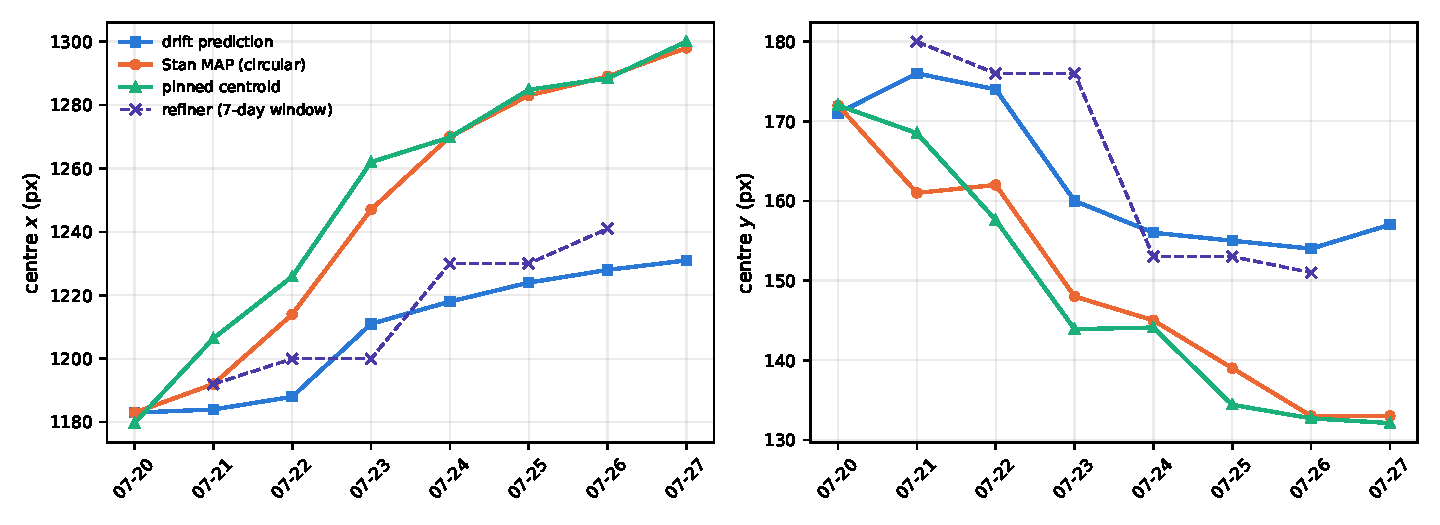
\includegraphics[width=\textwidth]{figs/tracks.pdf}
  \caption{Estimates of the blemish centre across eight days. The scene-drift prediction
  systematically lags: blemish motion is \emph{not} proportional to scene motion
  (\S\ref{sec:physics}). The Bayesian MAP track and the independent pinned-centroid
  track agree to $\sim\!\SI{3}{px}$ at both ends while sharing no machinery.}
  \label{fig:tracks}
\end{figure}

\section{The empirical transmittance map}
\label{sec:map}

The blemish's radial profile is not Gaussian: its wings fall faster than a Gaussian
matched at half depth (Figure~\ref{fig:profile}). The parametric blob is therefore used
only to \emph{locate}; depth and shape come from an empirical map,
\begin{equation}
  T_c(\mathbf{r}) \;=\; \operatorname{median}_j\,
     \frac{I_{j,c}(\mathbf{r})}{B_{j,c}(\mathbf{r})},
\end{equation}
the per-channel median, over selected frames, of each frame divided by its own quadratic
background, in linear light. Moving cloud averages out; fixed attenuation survives. Four
details matter:

\begin{itemize}
\item \textbf{Registration.} Each frame's window is extracted at that frame's
  velocity-interpolated centre, so the dip stacks aligned instead of being smeared by its
  motion across the stacking window.
\item \textbf{Blemish-local, sigma-clipped background rings.} The background is fitted on
  an annulus centred on the \emph{blemish} (never the window centre), with MAD-based
  outlier rejection; otherwise the dip leaks into its own background and the map records
  roughly half the true depth.
\item \textbf{Frame selection: bright first, then flat.} The dip is multiplicative, so
  signal scales with scene brightness. Selecting on flatness alone picks uniform
  overcast --- the flattest sky there is, and exactly where the dip sits at the noise
  floor.
\item \textbf{Edge-aware geometry.} The window is clamped to the frame --- the blemish
  sits closer to the top edge than the window half-size --- and the blemish's local
  coordinates inside the window, plus the measured centroid of the map's dip content,
  are published with the map. The corrector aligns the \emph{content}, never the window
  origin.
\end{itemize}

The publisher refuses to publish rather than publish junk: minimum frame counts per
channel and a sanity range on the map's peak depth. On any failure the live system keeps
the previous good map.

\begin{figure}[t]
  \centering
  \begin{subfigure}{0.47\textwidth}
    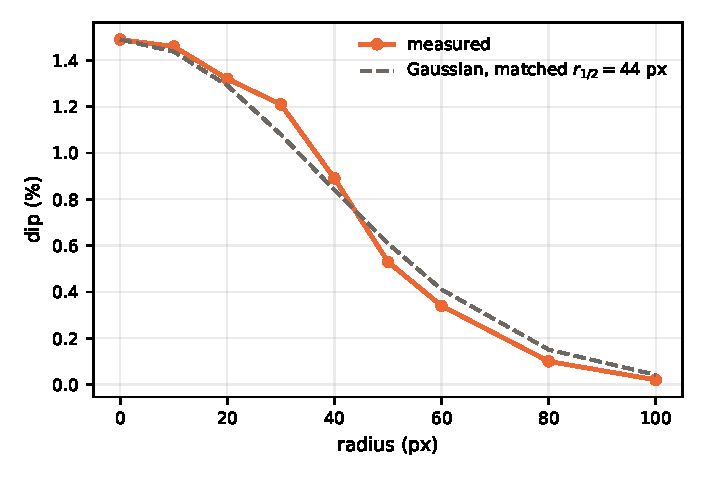
\includegraphics[width=\textwidth]{figs/profile.pdf}
    \caption{Measured radial profile vs.\ a Gaussian matched at half depth: the wings
    fall faster. Parametric fits locate; the empirical map corrects.}
    \label{fig:profile}
  \end{subfigure}\hfill
  \begin{subfigure}{0.49\textwidth}
    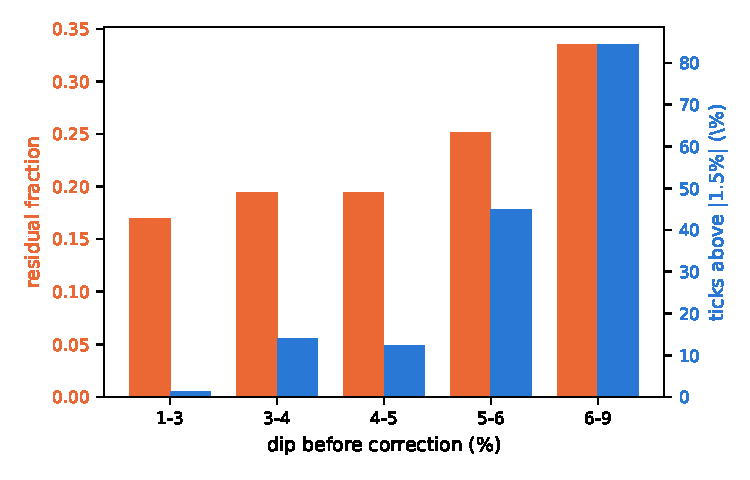
\includegraphics[width=\textwidth]{figs/gain_error.pdf}
    \caption{Why offline reprocessing solves its gain in display space: with a fixed
    linear-space gain, the residual is proportional to the input dip.}
    \label{fig:gain}
  \end{subfigure}
  \caption{Shape and gain measurements that fixed the design.}
\end{figure}

\section{Applying the correction}
\label{sec:apply}

\subsection{Position: three layers, fastest wins}

The blemish migrates intraday, so placement cannot rely on the nightly fit alone. At
every tick the corrector chains three estimators, each bounded by the one below it:

\begin{enumerate}
\item \textbf{Nightly posterior} (position, velocity, epoch) --- the slow, validated
  anchor.
\item \textbf{Velocity extrapolation} from the fit epoch to now (fractional days),
  total displacement capped at \SI{40}{px}.
\item \textbf{Persistent template lock} --- the measurement update. The corrector
  cross-correlates the frame's own dip (frame divided by its local background) against
  the map's dip template within $\pm\SI{25}{px}$; a decisive lock (normalised
  correlation $\ge 0.45$, clean surrounding ring) snaps the map onto the measured
  position \emph{and is saved}. A lock must also be unambiguous: the runner-up
  correlation peak (outside the winner's neighbourhood) must trail by a margin, so a
  cloud edge or contrail that ties the blemish cannot capture the tracker. The next tick
  starts from the last saved lock (if fresh and within \SI{40}{px} of the prediction)
  rather than from the prediction alone --- a tick-cadence recursive filter whose prior
  is minutes old instead of a day old. The nightly prediction remains the fallback and
  the sanity bound, so one corrupted lock cannot walk the correction away. The published
  bundle itself is integrity-checked on load (schema version, array hash, finiteness);
  a torn or corrupt publish is rejected and the previous state persists.
\end{enumerate}

The map content is placed by warping (bilinear, border transmittance $1.0$) with the
window origin fixed at its published, frame-clamped location --- necessary because the
blemish sits too close to the frame edge for the origin itself to follow it.

\subsection{Amplitude: exposure scaling plus gated self-calibration}

The map records depth at the reference exposure. Two mechanisms adapt it per frame:

\begin{itemize}
\item \textbf{Exposure scaling.} A measured depth-vs-level curve (fitted from
  within-tick bracket triples) scales the map's deficit by $s(L)/s_{\mathrm{ref}}$,
  where $L$ is the frame's local background level.
\item \textbf{Per-tick self-calibration, gated.} The tone curve is uncalibrated, so on
  dark backgrounds the true dip runs deeper than the scaled map. When the surrounding
  ring is clean enough to trust (relative MAD $<0.05$), the corrector measures the
  frame's own core deficit and trims the amplitude, clamped to $[0.75,1.35]\times$ the
  model. When the ring is cloudy the gate closes and the model amplitude stands ---
  chasing a cloud-inflated ``dip'' is how inverse bright spots are made.
\end{itemize}

The correction itself divides rather than reconstructs: $I \mapsto I/\tilde T$ with
$\tilde T$ feathered to unity outside the footprint, gain capped, and every corrected
pixel clamped never to exceed the local sky fit. Divide-only plus the cap makes an
inverse bright spot structurally impossible.

\subsection{Offline reprocessing: closed-loop gain}

For archive reprocessing, where four fusions per tick are affordable, the gain is solved
in \emph{display} space: fuse at two probe gains, take the secant step to the gain that
nulls the \emph{fused} dip, fuse once more. This removes all dependence on the
scene-dependent enhancement amplification (Figure~\ref{fig:gain}); the fitted gains
(median \num{2.83}) independently recover the measured $\approx\!2.85\times$ CLAHE
amplification.

\section{Physics: what the data established}
\label{sec:physics}

\paragraph{The image's motion is two-process --- but the object need not move.}
Step-level regression of daily blemish-image motion on scene drift (phase correlation on
the building band) gives
$\Delta x_{\text{image}} \approx 0.93\,\Delta x_{\text{scene}} + \epsilon$ with
$\operatorname{med}|\epsilon| \approx \SI{11}{px/day}$: camera rotation passes through
at unit gain, plus an independent component --- episodic, up to \SI{27}{px/day},
continuous within days (\SIrange{7}{18}{px}, measured by splitting days into thirds).
With the true shadow geometry (\S\ref{sec:what}) the independent component requires no
motion of the object at all: at $\sim\!\SI{3}{cm}$ standoff the lever arm is
$\sim\!\SI{92}{px}$ of image shift per millimetre of camera--pane relative translation,
so the entire week's \SI{120}{px} walk is \SI{1.3}{mm} of cumulative flexure, and the
intraday motion is \SIrange{0.08}{0.2}{mm} of thermal flex --- unremarkable for a
sun-struck sash with a camera resting against it. Day-by-day step ratios ranging from
$1.06$ to $26.7$ simply reflect days when the mount flexed without rotating and vice
versa. No constant ratio, and hence no feed-forward scheme, can track this; a
near-field fiducial (a tape dot on the glass) would separate camera flexure from any
residual object motion if the distinction ever matters. Operationally it does not: the
corrector tracks the apparent position either way.

\paragraph{A response-curve-confounded additive residual.} The slope of
equation~\eqref{eq:m1} is significantly nonzero in all channels and stable across nights
(blue $\approx +0.07$ at $p\sim10^{-9}$; green $+0.022$; red $+0.010$), strongly
chromatic (B$>$G$>$R by $\approx6.7\times$, a Rayleigh-like ordering). Its sign implies a
fixed \emph{dark} offset --- occlusion-like --- rather than added scattered light. Three
caveats mean this is exploratory, not established: the photometry aperture was fixed at
the original seed and drifted off the blemish for part of the record (it tracks the
published centre as of 2026-07-28, so future nights measure the feature itself); the
regression treats autocorrelated frames as independent; the linearisation is assumed
inverse-sRGB, and a tone-curve error generates exactly this signature; and one early
night shows the opposite sign. Until the response curve is calibrated per channel, the
term should be read as a response-curve-confounded residual rather than physics. The correction is
deliberately robust to the ambiguity: per-frame self-calibration corrects whatever depth
each exposure actually exhibits, without needing to know why.

\paragraph{Frame-edge geometry.} The blemish sits $\sim\!\SI{130}{px}$ below the frame
top while its background annulus extends to \SI{170}{px}: the ring is partially clipped
and the map window must be clamped (nothing can be cropped larger --- the frame is the
full sensor readout). Because the blemish is near-field, translating the camera up a few
millimetres would move it $\sim\!\SI{100}{px}$ down in frame while leaving the distant
framing essentially untouched; that remains the physical fix for edge margin, with the
caveat that migration continues regardless, so the tracker stays load-bearing.

\section{System architecture: where each computation runs}
\label{sec:architecture}

The system is two-tier by design (Figure~\ref{fig:flow}). Everything statistical and
expensive runs \emph{once per night} on a 32-core compute host (\code{akdeniz});
everything that runs \emph{per tick} is closed-form, operates on the published
$300\times300$ window rather than the \SI{4}{K} frame, and lives on the capture machine
(\code{pandr}, an M1 MacBook Air) inside the corrector itself. Measured on real frames,
the entire per-tick correction --- placement, template lock, amplitude calibration,
divide --- costs \SI{84}{ms} per bracket, about \SI{0.25}{s} of a \SIrange{15}{28}{s}
capture cycle.

\begin{table}[h]
\centering
\small
\footnotesize
\begin{tabular}{@{}p{6.6cm}lll@{}}
\toprule
level & where & cadence & cost \\
\midrule
MAP position/shape fit (multi-start L-BFGS) & \code{akdeniz} & nightly & seconds \\
registered transmittance map ($\sim$150 frames) & \code{akdeniz} & nightly & $\sim$\SI{2}{min} \\
acceptance validation (20 ticks $\times$ 4 fusions) & \code{akdeniz} & nightly & $\sim$\SI{4}{min} \\
publish (map $+$ model, $\sim$\SI{1.1}{MB}) & \code{akdeniz}$\to$\code{pandr} & nightly & seconds \\
per-tick correction (place, lock, calibrate, divide) & \code{pandr} & every tick & \SI{84}{ms}/bracket \\
archive reprocessing (closed-loop gain) & \code{akdeniz} & on demand & $\sim$\SI{7}{s}/tick, $26\times$ parallel \\
\bottomrule
\end{tabular}
\caption{Levels of computation. Only the nightly artifact crosses the network; the live
path has no per-tick dependency on the compute host.}
\label{tab:levels}
\end{table}

Two points about the split deserve emphasis. First, \textbf{the template lock is
computed on the Air, not on \code{akdeniz}}: it is part of the corrector, executed per
bracket on the local window --- two small Gaussian blurs and one
$120\times120$-in-$170\times170$ normalised cross-correlation, \SIrange{5}{10}{ms}. The
compute host never sees a live frame; its entire influence on the live system is the
nightly \code{spot\_model.json} $+$ \code{spot\_tmap.npy} pair. After the MAP fit,
nothing per-tick is an optimisation --- a warp, a correlation, two 6-parameter
least-squares fits, an elementwise divide.

Second, the split is about \emph{availability} as much as cost: the corrector sits in
the serving path, so a per-tick network dependency would turn any compute-host or
network outage into a real-time degradation of the public site. As built, \code{akdeniz}
can disappear for days: velocity extrapolation and the persistent lock carry the
placement, staleness tiers step down gracefully, and the acceptance gate catches any
quality regression when the nightly service resumes.

\begin{figure}[t]
\centering
\resizebox{\textwidth}{!}{%
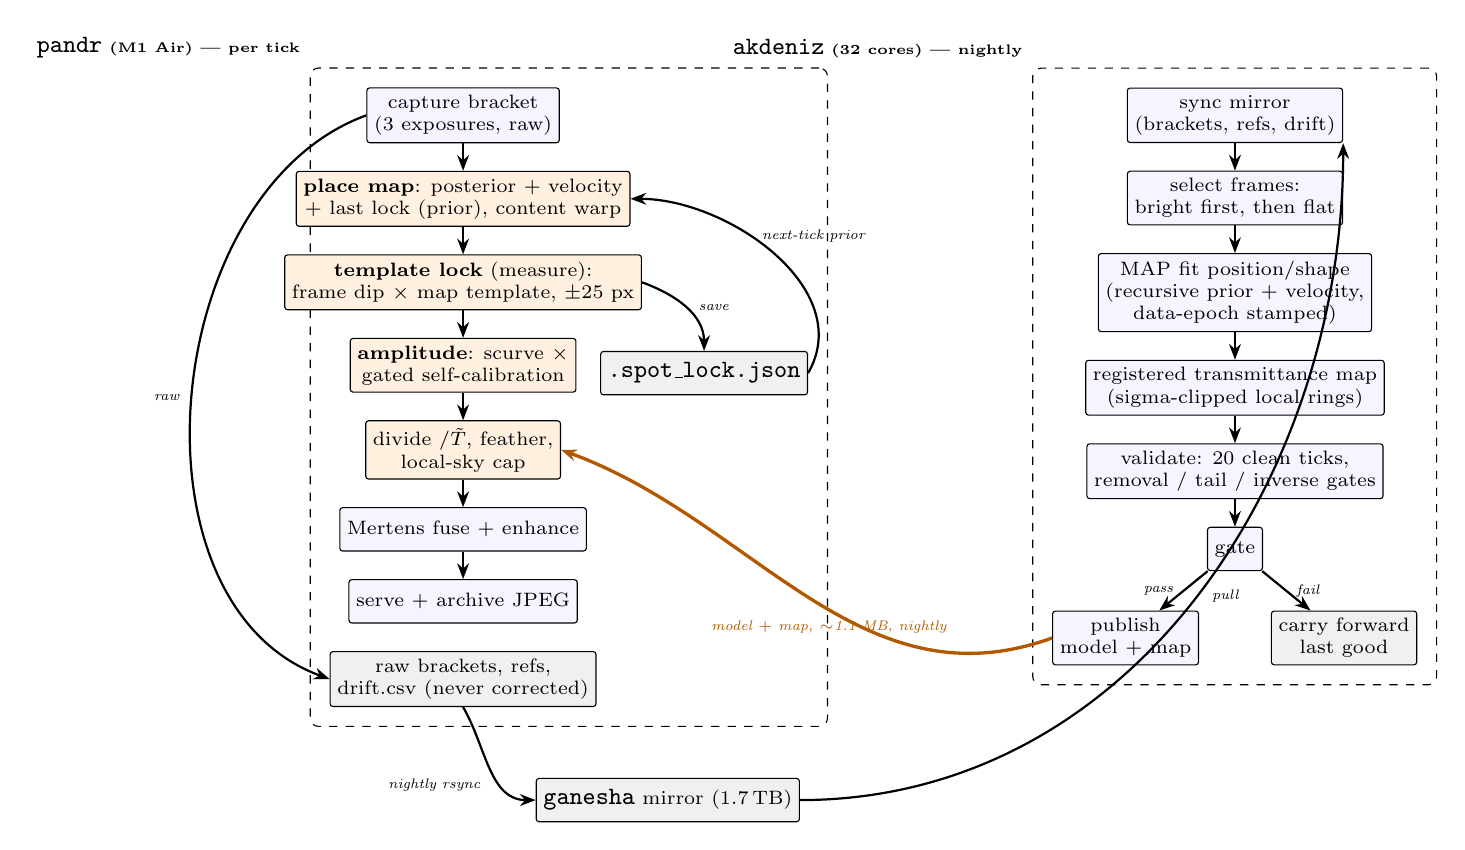
\begin{tikzpicture}[
  font=\scriptsize,
  node distance=3.5mm and 10mm,
  box/.style={draw, rounded corners=1pt, fill=blue!4, align=center,
              inner sep=2.6pt, minimum height=5.5mm},
  hot/.style={box, fill=orange!12},
  store/.style={box, fill=black!6},
  lane/.style={draw, dashed, rounded corners=3pt, inner sep=7pt},
  arr/.style={-{Stealth[length=2mm]}, thick},
  lbl/.style={font=\tiny\itshape, midway}
]
% ---- pandr lane (left) ----
\node[box]  (cap)  {capture bracket\\(3 exposures, raw)};
\node[hot,  below=of cap]  (place) {\textbf{place map}: posterior $+$ velocity\\
                                    $+$ last lock (prior), content warp};
\node[hot,  below=of place] (lock) {\textbf{template lock} (measure):\\
                                    frame dip $\times$ map template, $\pm$25 px};
\node[hot,  below=of lock]  (amp)  {\textbf{amplitude}: scurve $\times$\\
                                    gated self-calibration};
\node[hot,  below=of amp]   (div)  {divide $/\tilde T$, feather,\\local-sky cap};
\node[box,  below=of div]   (fuse) {Mertens fuse $+$ enhance};
\node[box,  below=of fuse]  (serve){serve $+$ archive JPEG};
\node[store, below=of serve] (raw) {raw brackets, refs,\\drift.csv (never corrected)};
\draw[arr] (cap) -- (place);
\draw[arr] (place) -- (lock);
\draw[arr] (lock) -- (amp);
\draw[arr] (amp) -- (div);
\draw[arr] (div) -- (fuse);
\draw[arr] (fuse) -- (serve);
\draw[arr] (cap.west) to[out=200, in=160] node[lbl, left=1pt]{raw} (raw.west);
% lock persistence self-loop
\node[store, right=3mm of amp, yshift=-1mm] (lockf) {\code{.spot\_lock.json}};
\draw[arr] (lock.east) to[out=-20, in=90] node[lbl, right=1pt]{save} (lockf.north);
\draw[arr] (lockf.east) to[out=60, in=0] node[lbl, right=1pt, pos=0.6]{next-tick prior} (place.east);
% ---- akdeniz lane (right) ----
\node[box, right=72mm of cap, xshift=0mm] (sync) {sync mirror\\(brackets, refs, drift)};
\node[box, below=of sync] (sel)  {select frames:\\bright first, then flat};
\node[box, below=of sel]  (map1) {MAP fit position/shape\\(recursive prior $+$ velocity,\\data-epoch stamped)};
\node[box, below=of map1] (reg)  {registered transmittance map\\(sigma-clipped local rings)};
\node[box, below=of reg]  (val)  {validate: 20 clean ticks,\\removal / tail / inverse gates};
\node[box, below=of val]  (gate) {gate};
\node[box, below left=5mm and 1mm of gate] (pub) {publish\\model $+$ map};
\node[store, below right=5mm and 1mm of gate] (keep) {carry forward\\last good};
\draw[arr] (sync) -- (sel);
\draw[arr] (sel) -- (map1);
\draw[arr] (map1) -- (reg);
\draw[arr] (reg) -- (val);
\draw[arr] (val) -- (gate);
\draw[arr] (gate) -- node[lbl, left]{pass} (pub);
\draw[arr] (gate) -- node[lbl, right]{fail} (keep);
% ---- cross-lane flows ----
\node[store, below=9mm of raw, xshift=26mm] (mirror) {\code{ganesha} mirror (\SI{1.7}{TB})};
\draw[arr] (raw.south) to[out=-60, in=180] node[lbl, below left]{nightly rsync} (mirror.west);
\draw[arr] (mirror.east) to[out=0, in=-90] node[lbl, right=2pt]{pull} (sync.south east);
\draw[arr, very thick, orange!70!black] (pub.west) to[out=200, in=-20]
     node[lbl, below, orange!70!black, pos=0.45]{model $+$ map, $\sim$1.1 MB, nightly} (div.east);
% ---- lane frames ----
\begin{scope}[on background layer]
\node[lane, fit=(cap)(serve)(raw)(lockf),
      label={[font=\tiny\bfseries]north west:{\code{pandr} (M1 Air) --- per tick}}] {};
\node[lane, fit=(sync)(gate)(pub)(keep),
      label={[font=\tiny\bfseries]north west:{\code{akdeniz} (32 cores) --- nightly}}] {};
\end{scope}
\end{tikzpicture}}
\caption{Data flow. Orange nodes run inside the corrector on the capture machine at
every tick; the template lock and its persistence loop are local to the Air. The compute
host's only influence on the live system is the nightly published model$+$map (orange
arrow); its only input is the raw-data mirror. Raw brackets and reference frames bypass
the corrector entirely, so the measurement stack is never contaminated by its own
correction.}
\label{fig:flow}
\end{figure}

\section{Autonomous operation}
\label{sec:autonomy}

A nightly job on \code{akdeniz} runs the whole cycle unattended: sync frames from the
mirror; select frames; fit the position (recursive prior, pinned across brackets); build
the registered maps; validate; publish to the capture host only if validation passes.
Validation runs on clean-sky ticks --- level and ring-structure thresholds measured
\emph{outside} the footprint, so the criterion cannot be circular --- and the gate
requires zero inverse spots, a floor on the median removal fraction, a bounded tail, and
no regression against a rolling baseline of recent accepted nights. Failure paths are
first-class: insufficient clear frames, low-confidence positions, and implausible jumps
all carry the previous parameters forward with a log line, and repeated failures
escalate. The corrector applies tiered staleness policies (beyond seven days it stands
down to a gated fallback). Success is asserted from output artifacts, never process exit
codes. Historical reprocessing uses the identical code path (\code{--replay}), which is
also the honest test of autonomy: replaying the archive exercises cold start,
carry-forward, gate rejections, and recovery exactly as a live outage would.

\section{Performance}
\label{sec:results}

\begin{figure}[t]
  \centering
  \begin{subfigure}{0.32\textwidth}
    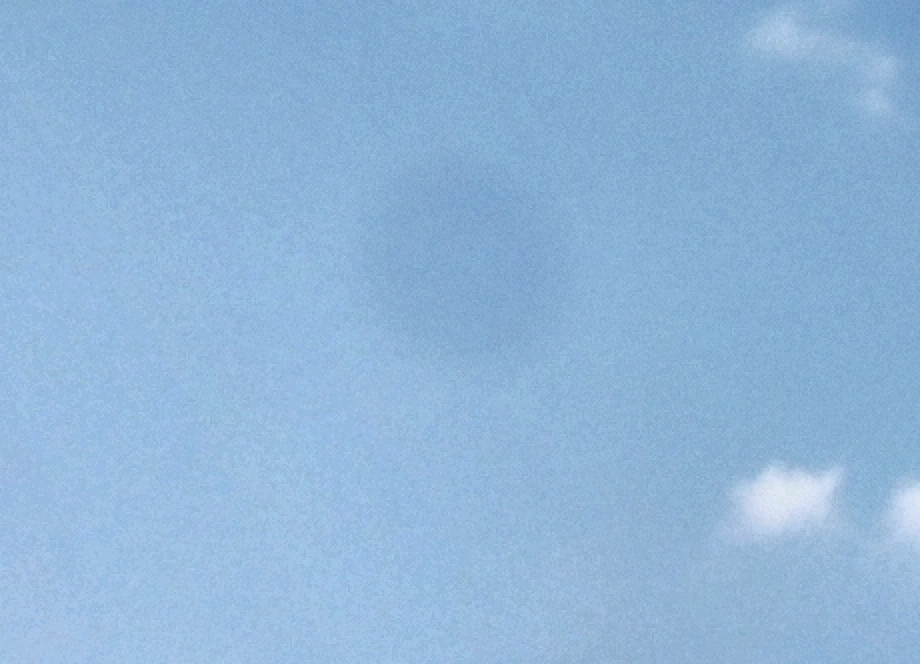
\includegraphics[width=\textwidth]{figs/before.png}\caption{before}
  \end{subfigure}\hfill
  \begin{subfigure}{0.32\textwidth}
    
\includegraphics[width=\textwidth]{figs/after.png}\caption{after}
  \end{subfigure}\hfill
  \begin{subfigure}{0.32\textwidth}
    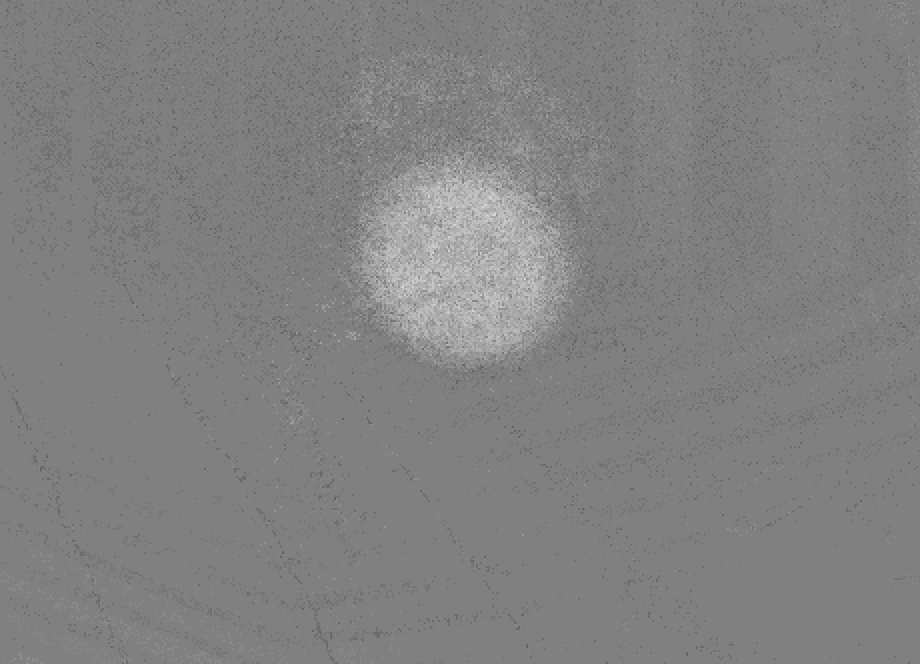
\includegraphics[width=\textwidth]{figs/diff.png}\caption{difference, $6\times$}
  \end{subfigure}
  \caption{Pixel-scale detail of the correction in Figure~\ref{fig:full}:
  \SI{4.49}{\percent} $\rightarrow$ \SI{0.60}{\percent}. The difference is a single
  compact blob; the cloud at lower right is untouched.}
  \label{fig:ba}
\end{figure}

\begin{table}[h]
\centering
\small
\begin{tabular}{lrrrrr}
\toprule
stratum (offline, closed-loop gain) & $n$ & before & after & removed & $|after|>1.5\%$ \\
\midrule
clean daylight frames & 495 & \SI{4.46}{\percent} & \SI{0.52}{\percent} & \SI{88.1}{\percent} & \SI{8.3}{\percent} \\
\quad + ring-structure gate & 301 & --- & \SI{0.51}{\percent} & --- & \SI{7.0}{\percent} \\
\bottomrule
\end{tabular}
\caption{Offline reprocessing statistics from \code{spot\_fit\_check/sweep2.csv}.
Selection, disclosed: displayed frame level $\ge 140$ and uncorrected measured dip in
$[1\%, 9\%]$ (row 2 adds ring-structure $< 3$). The dip window \emph{selects on a
measured quantity}: it estimates performance on frames where a blemish-scale dip is
detectable, and excludes negative, weak and cloud-inflated cases --- it is not a generic
daylight population. Residual distribution: 66 of 495 frames ($13\%$) end negative, six
below $-0.5\%$, one below $-1\%$ (minimum $-1.28\%$); ``inverse bright spot'' in the
text means a residual below $-1\%$. The 495 frames span 8 days
(\numrange{11}{111} per day); per-day median removal runs
\SIrange{83.2}{94.3}{\percent}, and a day-block bootstrap gives removal
\SI{88.1}{\percent} with 95\% CI $[\SI{85.6}{\percent}, \SI{90.9}{\percent}]$ and
median residual \SI{0.52}{\percent} with CI $[0.40, 0.66]$.}
\label{tab:strata}
\end{table}

Live evidence is retained in machine-readable form
(\code{spot\_paper/evidence/live\_paired.csv}: per tick, the served frame vs.\ a
re-fusion of its own raw brackets uncorrected, with positions, levels, ring structure
and model version). On the same clean-tick selection as Table~\ref{tab:strata}: the
clear evening of 07-27 gives $n=20$, median removal \SI{92.9}{\percent}, median served
residual \SI{+0.35}{\percent}, range $[-0.80, +1.44]$; 07-28 --- a heavily clouded day
during which the tracking chain was deployed and revised mid-day --- gives $n=13$
post-deployment clean ticks with median removal \SI{69.7}{\percent} and median residual
\SI{+1.70}{\percent}. The honest reading is that clear-sky live performance matches the
offline table and cloudy-sky ``clean'' ticks remain contaminated by weather at the
measurement aperture; a full clear-day out-of-sample evaluation is pending and the
evidence file will accumulate it. Centring is monitored separately by a dipole
statistic --- the signed difference between the dip in the leading and trailing
half-disks along the motion direction; a mis-centred correction is \emph{stationary}
and oriented, where cloud moves. After the epoch and measurement-update corrections this
statistic fell from $+2.5\%$ ($n=17$ frames) to $+0.4\%$ ($n=2$), with the remainder
symmetric weather signal.

\section{What is the blemish? A physical identification}
\label{sec:what}

The answer required one datum that no amount of image analysis could supply: the
camera's actual aperture. Two successive wrong identifications --- a migrating
condensation droplet, then a reflection of a room object --- were each internally
consistent with an \emph{assumed} webcam aperture of $f/2$--$f/2.4$. The published
specification for this camera is $f/4.0$, fixed focus at \SIrange{30}{120}{cm}: an
entrance pupil of $\approx\SI{1.1}{mm}$, not \SIrange{2.7}{3.9}{mm}. With that single
correction, every measurement converges on the mundane truth, which is also what direct
inspection of the pane suggests: \textbf{a $\sim\SI{0.25}{mm}$ speck of debris on the
glass}.

\paragraph{The solve.} A pixel viewing the distant scene collects a ray bundle that
crosses the pane as a patch of diameter $\approx a\,(1-d/F)$, where $d$ is the
pupil-to-pane distance and $F\approx\SI{0.5}{m}$ the fixed focus distance. A speck of
size $s$ removes the fraction $(s/a)^2$ of a pixel's light and images with full width
$\approx\big(s + a(1-d/F)\big)/d$. The measured depth (\SIrange{3}{7}{\percent}) gives
$s \approx 0.22a \approx \SI{0.24}{mm}$; the measured \SI{76}{px} FWHM then requires
$d \approx \SIrange{30}{35}{mm}$. Of that, at most $\sim\SI{13}{mm}$ is air gap and
glass, implying the entrance pupil sits $\sim\SI{2}{cm}$ behind the front of the lens
--- deep, but characteristic of short-focal-length inverted-telephoto designs, and a
checkable prediction. The faster-than-Gaussian wings (Figure~\ref{fig:profile}) are the
compact-support signature of exactly this: a hard-edged occluder convolved with a
hard-edged pupil. The neutral colour (integrated deficits equal across channels to
\SI{8}{\percent}; the red channel deeper but narrower, i.e.\ chromatic defocus, not
pigment) fits nondescript grey debris. The two or three fainter compact features
elsewhere on the pane are siblings: other motes.

\paragraph{Why the image moves.} The same geometry that blurs the speck amplifies
motion: image shift equals camera--pane translation divided by $d$, about
\textbf{\SI{92}{px/mm}}. The feature's entire week of ``migration'' (\SI{120}{px}) is
\SI{1.3}{mm} of accumulated flexure; its intraday drift is
\SIrange{0.08}{0.2}{mm} --- the thermal breathing of a sun-struck sash with a camera
resting against it. Nothing on the glass ever moved. The kinematic anomalies that
motivated more exotic identifications (episodic steps, opposite-signed step days, onset
with the hot spell) are all natural behaviours of \si{mm}-scale structural flexure seen
through a $30\times$ lever.

\paragraph{The colour of the blemish.} The registered per-channel transmittance maps
permit a measurement most defects never get: the speck's extinction spectrum, in three
bands. The subtlety is separating the \emph{object's} colour from the \emph{optics'}
colour --- longitudinal chromatic aberration gives each channel a slightly different
defocus blur, and a tighter point-spread function makes the same grey object look
deeper and narrower in that channel. The discriminator is the \emph{integrated}
deficit, $\int (1-T)\,dA$, which is invariant to blur:

\begin{center}
\small
\begin{tabular}{lccc}
\toprule
 & blue ($\sim$460 nm) & green ($\sim$540 nm) & red ($\sim$610 nm) \\
\midrule
core depth & \SI{4.49}{\percent} & \SI{4.89}{\percent} & \SI{5.38}{\percent} \\
half-depth radius & \SI{51.4}{px} & \SI{50.7}{px} & \SI{48.8}{px} \\
integrated deficit (rel.) & 1.00 & 1.08 & 1.07 \\
\bottomrule
\end{tabular}
\end{center}

Red is 20\% deeper than blue but also narrower, and the integrated deficits agree to
within 8\% across all three channels: the depth/width pattern is chromatic defocus (the
red PSF is slightly tighter for this near-field geometry), while the blur-invariant
total extinction is \textbf{neutral to $\pm 8\%$} --- with, if anything, a few percent
\emph{excess} extinction at the long-wavelength end, the opposite of Rayleigh-like
scattering. That bound excludes strongly pigmented candidates: rust ($\times$ several
in the blue), organic tar or sap, pollen, chlorophyll debris. What remains is the
unglamorous family that grey, wavelength-flat extinction describes: mineral dust,
paint or plaster fleck, paper fibre, insect frass. In transmission at $f/4$ the speck
is, to the limit of what three colour channels can say, \emph{grey} --- consistent with
the direct inspection finding an ordinary speck on the pane. (The blue-heavy
\emph{additive} residual of \S\ref{sec:physics} is a separate, response-curve-confounded
term and should not be read as the object's colour.)

\paragraph{Morals.} Three, earned expensively. First, \emph{an assumed instrument
parameter is a prior like any other, and a strong one}: two plausible physical stories
were built downstream of $f/2$, and both collapsed the moment the real $f/4$ was looked
up. Second, the apparent motion of a near-field feature is a strain gauge, not a
trajectory: at these standoffs the image measures \emph{mechanics} (of mount and sash)
more than it measures the object. Third, the correction architecture was right to track
the \emph{apparent} position agnostically --- every one of the candidate physical
stories moved the image the same way, and the corrector never needed to know which was
true. The remaining physical action item is pleasingly small: wipe the pane at the
predicted spot (inner surface first, then outer --- the \SI{3}{mm} path difference
changes the blur width measurably, so before-and-after even identifies which surface it
was on), and keep the tracker running for the next mote.

\section*{Code, data and reproducibility}

Deployed code is byte-copied under \code{production/} with a component-status table in
\code{PRODUCTION\_\allowbreak STATUS.md}. Offline analysis code (Stan models, drivers, map
builders, the intraday and colour measurements) is under \code{spot\_paper/code/};
evidence files are \code{spot\_fit\_\allowbreak check/sweep2.csv} (offline table, filters as
disclosed) and \code{spot\_paper/evidence/live\_paired.csv} (live paired
measurements). The synthetic end-to-end test (a frame carrying exactly the published
defect must null through the deployed corrector to $<0.5\%$) is
\code{tests/test\_synthetic\_\allowbreak end\_to\_end.py}; the current chain passes at
\SI{0.000}{\percent}. A fuller test matrix (edge-clamped crops, injected motion,
corrupted bundles, template-lock distractors) is specified in the 2026-07-28 review and
remains future work.

\section{Limitations}

\begin{itemize}
\item Live post-deployment evidence is one mixed-conditions day; the offline table is
  the strong result, and live parity is demonstrated only for one clear evening.
\item Cloudy-sky residuals at the blemish position are dominated by real cloud; the
  meaningful acceptance metric is clean-sky removal, and eye tests should distinguish
  stationary structure (defect) from structure that moves with the weather.
\item The acceptance metric shares its centre with the estimator; a common-mode position
  error would pass unnoticed. The population median of the uncorrected dip is the
  cross-check --- a mis-centred night reads visibly low.
\item The nightly state model is position-plus-velocity; intraday migration is handled
  by the template lock, not modelled. If migration accelerates beyond the
  $\pm\SI{25}{px}$ lock search radius within a day, tracking degrades gracefully to the
  prediction, and the gate catches the quality regression the next night.
\item The frame-edge geometry worsens at $\sim\!\SI{2}{px/day}$; the camera lift is
  physical maintenance that software cannot substitute for.
\item One-minute golden-hour frames keep no raw brackets, so their era corrections
  cannot be reprocessed; they are labelled rather than silently mixed with reprocessed
  frames.
\end{itemize}

\end{document}
